\documentclass[a4paper]{article}
\usepackage[T1]{fontenc}			% pacchetto per \chapter
\usepackage[italian]{babel}
\usepackage[italian]{isodate}  		% formato delle date in italiano
\usepackage{graphicx}				% gestione delle immagini
\usepackage{amsfonts}
\usepackage{booktabs}				% tabelle di qualità superiore
\usepackage{amsmath}				% pacchetto matematica
\usepackage{mathtools}				% per sottolineare sotto le equazioni
\usepackage{stmaryrd} 				% per '\llbracket' e '\rrbracket'
\usepackage{amsthm}					% teoremi migliorati
\usepackage{enumitem}				% gestione delle liste
\usepackage{pifont}					% pacchetto con elenchi carini
\usepackage{enumitem}				% pacchetto per elenchi con lettere dell'alfabeto
\usepackage{cancel}					% per cancellare delle espressioni matematiche
\usepackage{listings}				% implementa codice di programmazione


\usepackage[x11names]{xcolor}		% pacchetto colori RGB
% Link ipertestuali per l'indice
\usepackage{xcolor}
\usepackage[linkcolor=black, citecolor=blue, urlcolor=cyan]{hyperref}
\hypersetup{
	colorlinks=true
}

% Colour code style
\definecolor{codegreen}{rgb}{0,0.6,0}
\definecolor{codegray}{rgb}{0.5,0.5,0.5}
\definecolor{codepurple}{rgb}{0.58,0,0.82}
\definecolor{backcolour}{rgb}{0.95,0.95,0.92}

\lstdefinestyle{MATLAB}{
	backgroundcolor=\color{backcolour},   
	commentstyle=\color{codegreen},
	keywordstyle=\color{magenta},
	numberstyle=\tiny\color{codegray},
	stringstyle=\color{codepurple},
	basicstyle=\ttfamily\footnotesize,
	breakatwhitespace=false,         
	breaklines=true,                 
	captionpos=b,                    
	keepspaces=true,                 
	numbers=left,                    
	numbersep=5pt,
	showspaces=false,                
	showstringspaces=false,
	showtabs=false,                  
	tabsize=2
}
\lstset{style=MATLAB}

%\usepackage{showframe}				% visualizzazione bordi
%\usepackage{showkeys}				% visualizzazione etichetta

\newtheorem{theorem}{\textcolor{Red3}{\underline{Teorema}}}
\newtheorem{lemma}{Lemma}
\renewcommand{\qedsymbol}{QED}
\newcommand{\exec}[1]{\llbracket #1\:\rrbracket}
\newcommand{\dquotes}[1]{``#1''}
\newcommand{\longline}{\noindent\rule{\textwidth}{0.4pt}}

\begin{document}
	\author{Università degli Studi di Verona}
	\title{Simulazione di Elaborazione di segnali e immagini}
	\date{{\Large 29 Gennaio 2020}}
	\maketitle
	
	\section{Esercizio}
	
	Valutare graficamente il prodotto di convoluzione $y\left(t\right) = x\left(t\right) * h\left(t\right)$.
	
	\begin{figure}[!htp]
		\centering
		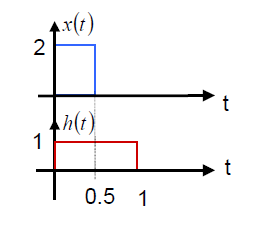
\includegraphics[width=.4\textwidth]{img/fig_1.png}
		\caption{Rappresentazione grafica del segnale $x\left(t\right)$ e $h\left(t\right)$.}
	\end{figure}
	
	\section{Esercizio}

	Valutare analiticamente o graficamente il prodotto di convoluzione $y\left(t\right) = x\left(t\right) * h\left(t\right)$.
	
	\begin{figure}[!htp]
		\centering
		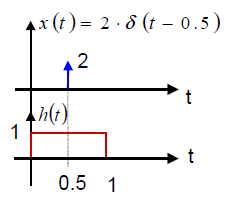
\includegraphics[width=.4\textwidth]{img/fig_2.png}
		\caption{Rappresentazione grafica del segnale $x\left(t\right)$ e $h\left(t\right)$.}
	\end{figure}

	\section{Esercizio}
	
	Dato il segnale $y\left(t\right)$, con trasformata di Fourier $Y\left(f\right)$ rappresentata in figura 3, rappresentare lo spettro $Yc\left(f\right)$ del segnale ottenuto campionando idealmente $y\left(t\right)$ con:
	\begin{enumerate}[label=\alph*)]
		\item $fc = 15 Hz$
		\item $fc = 17.5 Hz$
		\item $fc = 22 Hz$
	\end{enumerate}
	Determinare l'intervallo delle frequenze di aliasing nei tre casi appena elencati.\newline

	\noindent
	Nel caso \emph{a} determinare l'andamento del segnale campionato idealmente nel tempo $yc\left(t\right)$.
	
	\begin{figure}[!htp]
		\centering
		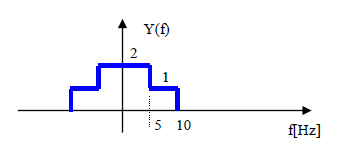
\includegraphics[width=.55\textwidth]{img/fig_3.png}
		\caption{Rappresentazione grafica del segnale $Y\left(f\right)$.}
	\end{figure}

	\section{Esercizio}
	
	Dato il risultato dell'esercizio precedente, determinare nei tre casi precedenti, lo spettro $Yr\left(f\right)$ del segnale all'uscita di un filtro di ricostruzione ideale, con risposta in frequenza $H\left(f\right)$ con frequenza di taglio:
	\begin{equation*}
		fp = \dfrac{fc}{2}
	\end{equation*}
	Determinare in quale dei tre casi si ricostruisce perfettamente il segnale continuo originario $y\left(t\right)$ e motivare la risposta.
\end{document}